\documentclass{article}
\usepackage[active,tightpage]{preview}
\renewcommand{\PreviewBorder}{1in}

\usepackage[english]{babel}
\usepackage{libertine}
\usepackage{libertinust1math}
\usepackage[T1]{fontenc}

\usepackage{graphicx}
\usepackage{caption}
\usepackage[autostyle]{csquotes}
\usepackage[style=authoryear,backend=biber]{biblatex}
\addbibresource{msredesign.bib}
\usepackage{hyperref}
\hypersetup{
    colorlinks=true,
    linkcolor=black,
    filecolor=black,
    urlcolor=black,
}
\urlstyle{same}


\title{msre design}
\author{aslak stubsgaard}
\date{}

\usepackage{lipsum}
\begin{document}
\begin{preview}
\maketitle

\section{introduction}
the design and dimensions of the molten salt reactor experiment is detailed in several ornl reports. this document aims at providing a comprehensive overview of the core design dimensions and materials, for the purpose of creating an accurate cad model of the reactor.
care is taken to give proper references to where data comes from or how its extrapolated from the available information.

\section{core design}
the msre core design can be seen in figure 1 and figure 2, note that they differ slight, e.g. the vessel drain line and around the control rod.
\begin{center}
  \fbox{\includegraphics[page=5,width=0.8\textwidth,trim={2cm 6cm 3.5cm 4cm},clip]{./references/ORNL-TM-3229.pdf}}\\
  figure 1: MSRE reactor vessel \parencite[figure 1]{ornl-tm-3229}.
\end{center}
\begin{center}
  \fbox{\includegraphics[page=9,width=0.8\textwidth,trim={4cm 4cm 2.5cm 3cm},clip]{./references/ORNL-TM-0378.pdf}}\\
  figure 2: cutaway drawing of IGRE core and core vessel \parencite[figure 1]{ornl-tm-0378}.
\end{center}


\subsection{control rod and sample assembly}
the control rod and sample assembly is further detailed in figure 3.
\begin{center}
  \fbox{\includegraphics[page=10,width=0.8\textwidth,trim={3cm 9.5cm 3.5cm 8cm},clip]{./references/ORNL-TM-0378.pdf}}\\
  figure 3: msre control rod arrangements and typical fuel channels \parencite[figure 2]{ornl-tm-0378}.
\end{center}


\section{graphite rods}
the graphite moderator rod dimension, given in figure 4, are missing the angle of the spike, the dimensions of the pole, and disk at the bottom.
\begin{center}
  \centering
  \fbox{\includegraphics[page=6,width=0.8\textwidth,trim={3.5cm 6cm 2.5cm 5cm},clip]{./references/ORNL-TM-3229.pdf}}\\
  figure 4: typical graphite core block arrangement \parencite[figure 2]{ornl-tm-3229}.
\end{center}

the arangement of the graphite rods are detailed in figure 5
\begin{center}
  \centering
  \fbox{
  \includegraphics[page=10,width=0.42\textwidth,trim={1cm 3cm 0.25cm 4cm},clip]{./references/ORNL-TM-4174.pdf}
  \hspace{-0.2cm}
  \includegraphics[page=11,width=0.36\textwidth,trim={2cm 3.1cm 3cm 4cm},clip]{./references/ORNL-TM-4174.pdf}
  }\\
  figure 5: reactor core block assembly plan, drawing D-BB-B-40416 \parencite[page 10-11]{ornl-tm-4174}.
\end{center}


\printbibliography

\end{preview}
\end{document}
